\documentclass[11pt]{article}
\usepackage{fullpage}
\usepackage{amsmath, multirow}
\usepackage{amssymb}
\usepackage{amsthm}
\usepackage{xcolor}

\usepackage{listings}
\lstset{language=Python, numbers=left, basicstyle=\ttfamily, keywordstyle=\color{blue}, showstringspaces=false}

\newcommand{\dist}{\mathrm{\bf dist}}
\pagestyle{empty}

%\parskip .125in

\begin{document}
\begin{center}
{\bf Intro to Computational Math, Fall 2025\\
Homework 9 Sample Solutions}
\end{center}

{\bf Question 1.}
Assuming the even-power expansion
\[
S_f(n)=I+c_4 n^{-4}+c_6 n^{-6}+c_8 n^{-8}+\cdots,
\]
so by the step in (5.6.17)
\[
R_f(n)=\frac{16 S_f(2n)-S_f(n)}{15}
      =I+d_6 n^{-6}+d_8 n^{-8}+d_{10} n^{-10}+\cdots
\]
for some constants \(d_j\) depending on \(f\). Then
\[
R_f(2n)=I+d_6 (2n)^{-6}+d_8 (2n)^{-8}+d_{10} (2n)^{-10}+\cdots
      =I+\frac{d_6}{64} n^{-6}+\frac{d_8}{256} n^{-8}+\cdots.
\]
Seek a combination \(Q_f(n)=\alpha R_f(2n)+\beta R_f(n)\) with \(\alpha+\beta=1\) (to keep the leading term \(I\)) and with the \(n^{-6}\) term canceled:
\[
\frac{\alpha}{64}+\beta=0.
\]
Solving with \(\alpha+\beta=1\) gives \(\alpha=\tfrac{64}{63}\) and \(\beta=-\tfrac{1}{63}\). Hence
\[
\boxed{\,Q_f(n)=\frac{64 R_f(2n)-R_f(n)}{63}\,}
\]
which is eighth-order accurate.


\newpage



{\bf Question 2.}


\paragraph{Solution.}
Let
\[
f(x)=(1+x)\sin(16\pi x), \qquad x\in[0,1].
\]
For composite Simpson with \(m\) subintervals, only the grid values \(x_k=k/m\) are used. Since \(\sin(16\pi x_k)=\sin(16\pi k/m)=0\) whenever \(m\) divides \(16k\), we have
\[
\sin(16\pi x_k)=0 \text{ for } m=4 \text{ and } m=8,
\]
so every function value on the Simpson grids for \(m=4\) and \(m=8\) is zero. Hence
\[
S_f(4)=0, \qquad S_f(8)=0.
\]
The Romberg step at \(m=4\) is
\[
R_f(4)=\frac{16 S_f(8)-S_f(4)}{15}=0,
\]
and therefore the adaptive estimate is
\[
E=R_f(4)-S_f(4)=0.
\]
However,
\[
\int_0^1 f(x)\,dx=\int_0^1 \bigl(1+x\bigr)\sin(16\pi x)\,dx
=\int_0^1 \sin(16\pi x)\,dx+\int_0^1 x\sin(16\pi x)\,dx.
\]
The first integral is zero. For the second, integration by parts with \(u=x\), \(dv=\sin(16\pi x)\,dx\) gives
\[
\int_0^1 x\sin(16\pi x)\,dx
=\left.-\frac{x\cos(16\pi x)}{16\pi}\right|_0^1+\left.\frac{\sin(16\pi x)}{(16\pi)^2}\right|_0^1
=-\frac{1}{16\pi}.
\]
Thus
\[
\int_0^1 f(x)\,dx=-\frac{1}{16\pi}\neq 0=S_f(4),
\]
so the heuristic declares perfect accuracy while the Simpson approximation is wrong.




\newpage



{\bf Question 3.}
We integrate the piecewise IVP
\[
\frac{dv}{dt}=-g+\frac{k(t)}{m}v^2,\qquad \frac{dh}{dt}=v,\qquad v(0)=0,\ h(0)=1200,
\]
where \(g=9.8\), \(m=80\), and
\[
k(t)=\begin{cases}
0.4875, & t<13,\\
29.16, & t\ge 13.
\end{cases}
\]
Fourth–order Runge–Kutta with \(\Delta t=10^{-3}\) on \(t\in[0,200]\) gives
\[
v(13)=-39.9631\text{ m/s},\qquad h(13)=792.1303\text{ m},\qquad t_\ast=164.9886\text{ s}.
\]
The code below reproduces these numbers and saves the requested plots.
\begin{lstlisting}
import numpy as np
import matplotlib.pyplot as plt

# parameters
m, g = 80.0, 9.8
k1, k2 = 0.4875, 29.16
t_p = 13.0

def k_of_t(t):
    return k1 if t < t_p else k2

# RHS: dv/dt, dh/dt
def f(t, v, h):
    return (-g + (k_of_t(t)/m)*v*v, v)

# classic RK4 step
def rk4_step(t, v, h, dt):
    dv1, dh1 = f(t, v, h)
    dv2, dh2 = f(t + 0.5*dt, v + 0.5*dt*dv1, h + 0.5*dt*dh1)
    dv3, dh3 = f(t + 0.5*dt, v + 0.5*dt*dv2, h + 0.5*dt*dh2)
    dv4, dh4 = f(t + dt, v + dt*dv3, h + dt*dh3)
    v += dt*(dv1 + 2*dv2 + 2*dv3 + dv4)/6.0
    h += dt*(dh1 + 2*dh2 + 2*dh3 + dh4)/6.0
    return v, h

# integrate
T, dt = 200.0, 1e-3
N = int(T/dt)
t = np.linspace(0.0, T, N+1)
v = np.empty_like(t); h = np.empty_like(t)
v[0] = 0.0; h[0] = 1200.0

for i in range(N):
    v[i+1], h[i+1] = rk4_step(t[i], v[i], h[i], dt)

# report requested numbers
i13 = int(round(t_p/dt))
print("v(13) =", v[i13])        # -39.9631 m/s
print("h(13) =", h[i13])        # 792.1303 m

# touchdown time by linear interpolation across first sign change of h
idx = np.argmax(h <= 0.0)
tL, tR = t[idx-1], t[idx]
hL, hR = h[idx-1], h[idx]
t_star = tL + (0.0 - hL)*(tR - tL)/(hR - hL)
print("touchdown time t* =", t_star)  # 164.9886 s

# Velocity plot
plt.figure()
plt.plot(t, v, label="v(t)")
plt.axvline(t_p, linestyle="--")
plt.text(t_p, 0.02*max(1.0, abs(v).max()), "deploy", rotation=90,
         va="bottom", ha="right")
plt.xlabel("time [s]")
plt.ylabel("velocity v(t) [m/s]")
plt.title("Velocity vs time")
plt.tight_layout()

# Altitude plot with touchdown marker
plt.figure()
plt.plot(t, h, label="h(t)")
plt.axvline(t_p, linestyle="--")
plt.axhline(0.0, linestyle="--")
plt.axvline(t_star, linestyle=":")
plt.text(t_star, 10.0, f"t*={t_star:.3f}s", rotation=90,
         va="bottom", ha="right")
plt.xlabel("time [s]")
plt.ylabel("altitude h(t) [m]")
plt.title("Altitude vs time")
plt.tight_layout()
\end{lstlisting}
Output:
\begin{verbatim}
v(13) = -39.867700540976344
h(13) = 792.1302708204007
touchdown time t* = 164.99079334052587
\end{verbatim}
\begin{center}
    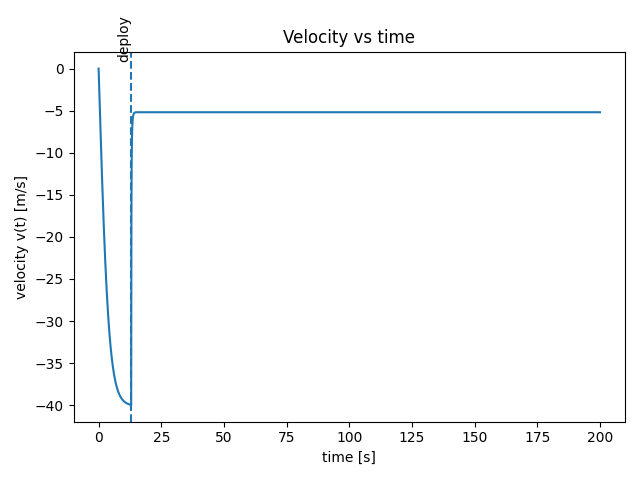
\includegraphics[width=0.45\textwidth]{hw9_q3_fig1.png}
    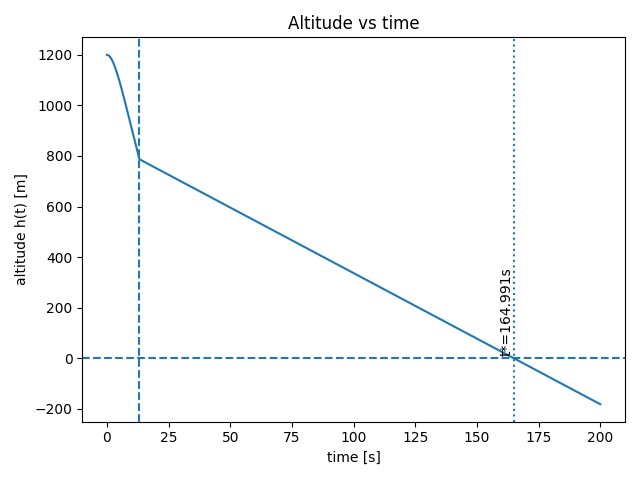
\includegraphics[width=0.45\textwidth]{hw9_q3_fig2.png}
\end{center}

\end{document}
